\documentclass{article}

% Language setting
% Replace `english' with e.g. `spanish' to change the document language
\usepackage[english]{babel}

% Set page size and margins
% Replace `letterpaper' with `a4paper' for UK/EU standard size
\usepackage[letterpaper,top=2cm,bottom=2cm,left=3cm,right=3cm,marginparwidth=1.75cm]{geometry}

% Useful packages
\usepackage{amsmath}
\usepackage{graphicx}
\usepackage[colorlinks=true, allcolors=blue]{hyperref}

\title{TDT4171 — Artificial Intelligence Methods \\ Assignment 7 - Neural Networks Intro}
\author{Erik Storås Sommer - 535006}
\date{March 2023}

\begin{document}
\maketitle
\setlength{\parindent}{0pt}

\section*{Feedforward Neural Network}

The hyperparameters used for the neural network are shown in Figure \ref{fig:image1}.
The weights and biases in the network is tuned using the gradient descent algorithm, and the loss function is the mean squared error.
The network is trained for 100000 epochs, and the learning rate is set to 0.0001.
Tried different epochs and learning rates, and found that these values gave the best results.

\begin{figure}[hbtp]
    \centering
    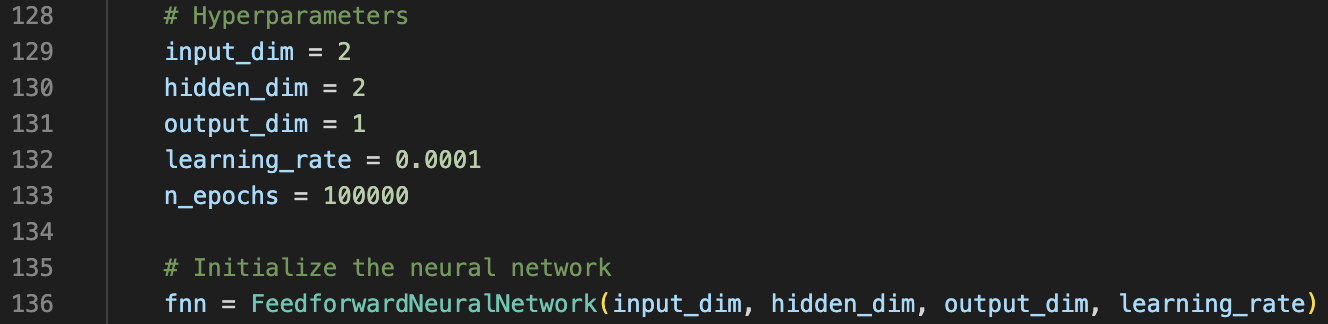
\includegraphics[width=0.8\textwidth]{hyperparameters.png}
    \caption{Hyperparameters used for the neural network}
    \label{fig:image1}
\end{figure}

The output from running the attached python file is shown in Figure \ref{fig:image2}.
The output for the loss function is gradually decreasing as the network is trained, hinting that the network is learning.
To se the performance of the network, the mean squared error for the train and test set is calculated and printed before and after training.
As shown in the output, the mean squared error for the train set is $\approx$ 0.126, and the mean squared error for the test set is $\approx$ 0.13, both after training.
This means that the network is able to generalize well, and is not overfitting the data.

\begin{figure}[hbtp]
    \centering
    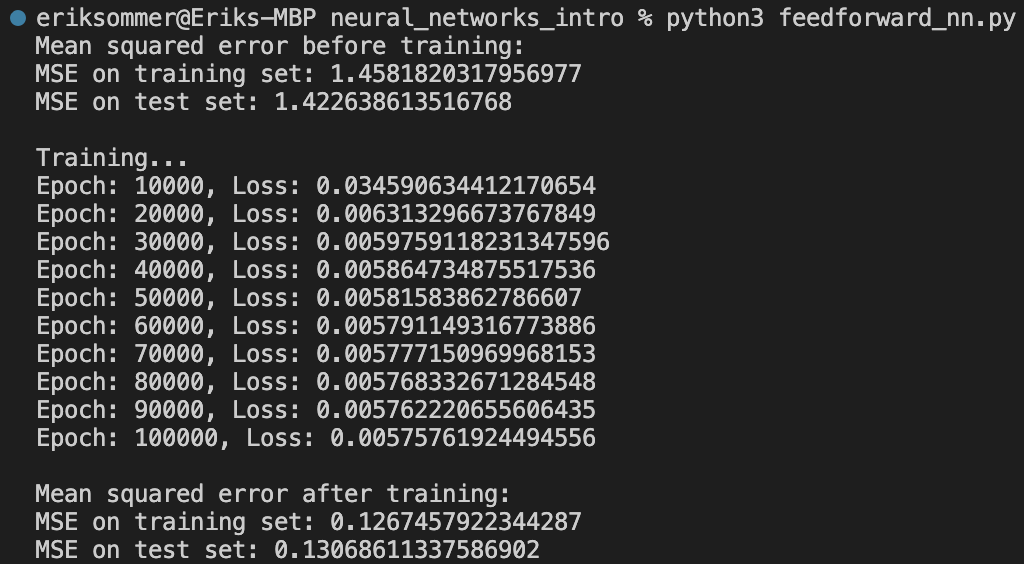
\includegraphics[width=0.8\textwidth]{output.png}
    \caption{Output from running the attached python file}
    \label{fig:image2}
\end{figure}

\end{document}